\documentclass{article}
\usepackage{tikz}


\begin{document}

\begin{tikzpicture}

\begin{scope}[inner sep=0pt]
    \node (v) at (3,-2) {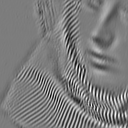
\includegraphics[scale=0.25]{generative.png}};
    \node (data) at (0,-2) {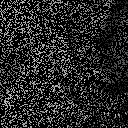
\includegraphics[scale=0.25]{data.png}};
    \node (u) at (6,-2) {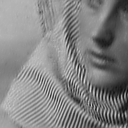
\includegraphics[scale=0.25]{reconstructed.png}};
    
    
    \node[fill=black] (00) at (0,-3.25) {};
    \node[fill=black] (01) at (2,-3.25) {};
    \node[fill=black] (02) at (3,-3.25) {};
    \node[fill=black] (03) at (4,-3.25) {};
    \node[fill=black] (04) at (6,-3.25) {};
    
    
    \node (k00) at (0,-4) {
\includegraphics[scale=1]{kernel_0_0.png}};
    \node (k01) at (2,-4) {
\includegraphics[scale=1]{kernel_0_1.png}};
    \node (k03) at (4,-4) {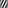
\includegraphics[scale=1]{kernel_0_3.png}};
    \node (k04) at (6,-4) {
\includegraphics[scale=1]{kernel_0_4.png}};
    
    \node (l00) at (0,-5) {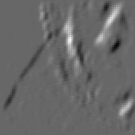
\includegraphics[scale=0.25]{latent_0_0.png}};
    \node (l01) at (2,-5) {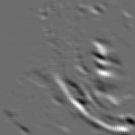
\includegraphics[scale=0.25]{latent_0_1.png}};
    \node (l03) at (4,-5) {
\includegraphics[scale=0.25]{latent_0_3.png}};
    \node (l04) at (6,-5) {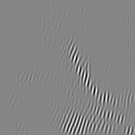
\includegraphics[scale=0.25]{latent_0_4.png}};
    
    \node (k10) at (0,-6.25) {
\includegraphics[scale=1]{kernel_1_0.png}};
    \node (k11) at (2,-6.25) {
\includegraphics[scale=1]{kernel_1_1.png}};
    \node (k13) at (4,-6.25) {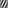
\includegraphics[scale=1]{kernel_1_3.png}};
    \node (k14) at (6,-6.25) {
\includegraphics[scale=1]{kernel_1_4.png}};
    
    \node (l10) at (0,-7) {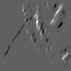
\includegraphics[scale=0.25]{latent_1_0.png}};
    \node (l11) at (2,-7) {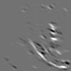
\includegraphics[scale=0.25]{latent_1_1.png}};
    \node (l13) at (4,-7) {
\includegraphics[scale=0.25]{latent_1_3.png}};
    \node (l14) at (6,-7) {
\includegraphics[scale=0.25]{latent_1_4.png}};
    
    \node (k20) at (0,-8) {
\includegraphics[scale=1]{kernel_1_0.png}};
    \node (k21) at (2,-8) {
\includegraphics[scale=1]{kernel_1_1.png}};
    \node (k23) at (4,-8) {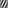
\includegraphics[scale=1]{kernel_1_3.png}};
    \node (k24) at (6,-8) {
\includegraphics[scale=1]{kernel_1_4.png}};
    
    \node (l20) at (0,-8.75) {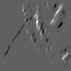
\includegraphics[scale=0.25]{latent_1_0.png}};
    \node (l21) at (2,-8.75) {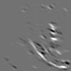
\includegraphics[scale=0.25]{latent_1_1.png}};
    \node (l23) at (4,-8.75) {
\includegraphics[scale=0.25]{latent_1_3.png}};
    \node (l24) at (6,-8.75) {
\includegraphics[scale=0.25]{latent_1_4.png}};
    
    
\end{scope}
    
    \path [-] (data) edge (v);
    \path [->] (v) edge (u);
    \path [->] (02) edge (v);
    
    \path [-] (00) edge (02);
    \path [-] (01) edge (02);
    \path [-] (03) edge (02);
    \path [-] (04) edge (02);
    
    \draw [-] (k00) -- (00) -- (02);
    \path [-] (k01) edge (01);
    \path [-] (k03) edge (03);
    \path [-] (k04) edge (04);
    
	\path [-] (l00) edge (k00);
    \path [-] (l01) edge (k01);
    \path [-] (l03) edge (k03);
    \path [-] (l04) edge (k04);
    
    \path [->] (k10) edge (l00);
    \path [->] (k11) edge (l01);
    \path [->] (k13) edge (l03);
    \path [->] (k14) edge (l04);
    
    \path [-] (l10) edge (k10);
    \path [-] (l11) edge (k11);
    \path [-] (l13) edge (k13);
    \path [-] (l14) edge (k14);
    
    \path [->] (k20) edge (l10);
    \path [->] (k21) edge (l11);
    \path [->] (k23) edge (l13);
    \path [->] (k24) edge (l14);
    
    \path [-] (l20) edge (k20);
    \path [-] (l21) edge (k21);
    \path [-] (l23) edge (k23);
    \path [-] (l24) edge (k24);

% 
%    \path [->](11) edge node [style={pos=.25}] {$*\theta^1_{1}$} (sum);
%    \path [->](12) edge node [style={pos=.25}] {$*\theta^1_{n}$} (sum);
%    \path [->](13) edge node [style={pos=.25}] {$*\theta^1_{N}$} (sum);
%    \path [->](sum) edge (v);


\end{tikzpicture}

\end{document}